\documentclass{beamer}
\usepackage[utf8]{inputenc}

\usetheme{Madrid}
\usecolortheme{default}
\usepackage{extarrows}
\usepackage{amsmath}
\usepackage{extarrows}
\usepackage{amssymb,amsfonts,amsthm}
\usepackage{txfonts}
\usepackage{tkz-euclide}
\usepackage{listings}
\usepackage{adjustbox}
\usepackage{array}
\usepackage{tabularx}
\usepackage{gvv}
\usepackage{lmodern}
\usepackage{circuitikz}
\usepackage{tikz}
\usepackage{graphicx}
\usepackage{amsmath} 

\setbeamertemplate{page number in head/foot}[totalframenumber]

\usepackage{tcolorbox}
\tcbuselibrary{minted,breakable,xparse,skins}

\definecolor{bg}{gray}{0.95}
\DeclareTCBListing{mintedbox}{O{}m!O{}}{%
  breakable=true,
  listing engine=minted,
  listing only,
  minted language=#2,
  minted style=default,
  minted options={%
    linenos,
    gobble=0,
    breaklines=true,
    breakafter=,,
    fontsize=\small,
    numbersep=8pt,
    #1},
  boxsep=0pt,
  left skip=0pt,
  right skip=0pt,
  left=25pt,
  right=0pt,
  top=3pt,
  bottom=3pt,
  arc=5pt,
  leftrule=0pt,
  rightrule=0pt,
  bottomrule=2pt,
  toprule=2pt,
  colback=bg,
  colframe=orange!70,
  enhanced,
  overlay={%
    \begin{tcbclipinterior}
    \fill[orange!20!white] (frame.south west) rectangle ([xshift=20pt]frame.north west);
    \end{tcbclipinterior}},
  #3,
}
\lstset{
    language=C,
    basicstyle=\ttfamily\small,
    keywordstyle=\color{blue},
    stringstyle=\color{orange},
    commentstyle=\color{green!60!black},
    numbers=left,
    numberstyle=\tiny\color{gray},
    breaklines=true,
    showstringspaces=false,
}
\title %optional
{8.4.35}


\author 
{Kartik Lahoti - EE25BTECH11032}



\begin{document}


\frame{\titlepage}
\begin{frame}{Question}
The ellipse $E_1\colon\frac{x^2}{9}+\frac{y^2}{4} = 1$ is inscribed in a rectangle \textbf{R} whose sides are parallel to coordinate axes. another ellipse $E_2$ passing through the point $\brak{0,4}$ circumscribes the rectangle \textbf{R}. The eccentricity of the ellipse $E_2$ is 
 \begin{multicols}
    \begin{enumerate}       
        \item $\frac{\sqrt{2}}{2}$
        \item $\frac{\sqrt{3}}{2}$
        \item $\frac{1}{2}$
        \item $\frac{3}{4}$        
    \end{enumerate}
\end{multicols}
\end{frame}

\begin{frame}{Theoretical Solution}
Given for $E_1\colon$

\begin{table}[H]
    \centering
    \begin{tabular}{|c|c|}
\hline
\textbf{Name} & \textbf{Value} \\ \hline
$\vec{A}$ & $\myvec{2 & 1 \\0 & 3}$ \\ \hline
\end{tabular}

    \caption{8.4.35}
    \label{tab:placeholder}
\end{table}

\end{frame}

\begin{frame}{Theoretical Solution}
    $E_1$ is inscribed in Rectangle
    
    $\therefore$ The coordinates of Vertices of Rectangles are intersection points of, 
    
    \begin{align}
        \vec{e_1}^{\top}\vec{x} &= 3 \label{eq_1} \\ 
        \vec{e_2}^{\top}\vec{x} &= 2 \label{eq_2} \\ 
        \vec{e_1}^{\top}\vec{x} &= -3\\
        \vec{e_2}^{\top}\vec{x} &= -2
    \end{align}
    
    Let $\vec{P}$ intersection of \ref{eq_1} and \ref{eq_2}, 
    \begin{align}
        \vec{P} = \myvec{3\\2}
    \end{align}
    
    Let , 
    \begin{align}
        \vec{Q} = \myvec{0\\4}
    \end{align}
\end{frame}

\begin{frame}{Theoretical Solution}
    General Form of Conic equation is given as , 
    
    \begin{align}
        g\brak{\vec{x}} = \vec{x}^{\top}\vec{V}\vec{x} + 2\vec{u}^{\top}\vec{x} + f = 0 
    \end{align}
    
    Since the rectangle in inscribed inside $E_2$ , $E_2$ is an ellipse centered at origin. 
    
    For a conic centered at Origin 
    \begin{align}
        \vec{u} = \vec{0}    
    \end{align}
    
    \begin{align}
        \therefore \vec{x}^{\top}\vec{V^{\prime}}\vec{x} = 1  \label{eq_3}
    \end{align}
    
    where, $\vec{V^{\prime}} = -\frac{1}{f}\vec{V}$
\end{frame}

\begin{frame}{Theoretical Solution}

    Since $E_2$ has axes parallel to coordinate axes , $\vec{V^{\prime}}$ must be diagonal.
    
    \begin{align}
        \vec{V^{\prime}} = \myvec{v_{11} & 0 \\ 0 & v_{22}}
    \end{align}
    
    Now, $E_2$ passes through $\vec{Q}$ and $\vec{P}$
    
    \begin{align}
        \vec{Q}^{\top}\vec{V^{\prime}}\vec{Q} = 1 \\ 
        \vec{P}^{\top}\vec{V^{\prime}}\vec{P} = 1 
    \end{align}
\end{frame}
\begin{frame}{Theoretical Solution}
    we get following system of eqn , 
    \begin{align}
        \myvec{9 & 4 }\myvec{v_{11} \\ v_{22}} = 1    
    \end{align}
    
    \begin{align}
        \myvec{0 & 16 }\myvec{v_{11} \\ v_{22}} = 1    
    \end{align}
\end{frame}

\begin{frame}{Theoretical Solution}
\begin{align}
    \augvec{2}{1}{9 & 4 & 1\\0 & 16 & 1}\xleftrightarrow[]{R_1\rightarrow \frac{R_1}{9}}\augvec{2}{1}{1 & \frac{4}{9} & \frac{1}{9}\\0 & 16 & 1}
\end{align}

\begin{align}
    \augvec{2}{1}{1 & \frac{4}{9} & \frac{1}{9}\\0 & 16 & 1}\xleftrightarrow[]{R_2\rightarrow \frac{R_2}{16}}\augvec{2}{1}{1 & \frac{4}{9} & \frac{1}{9}\\0 & 1 & \frac{1}{16}}
\end{align}
\end{frame}

\begin{frame}{Theoretical Solution}
\begin{align}
    \augvec{2}{1}{1 & \frac{4}{9} & \frac{1}{9}\\0 & 1 & \frac{1}{16}}\xleftrightarrow[]{R_1\rightarrow R_1 - \frac{4}{9}R_2}\augvec{2}{1}{1 & 0 & \frac{1}{12}\\0 & 1 & \frac{1}{16}}
\end{align}

On solving , We get

\begin{align}
    \vec{V^{\prime}} = \myvec{\frac{1}{12} & 0 \\ 0 & \frac{1}{16}}
\end{align}

\begin{align}
    \vec{V} = \norm{n}^2\vec{I} - e^2\vec{n}^{\top}\vec{n}
\end{align}

Here, $\vec{n} = \vec{e_2}$
\end{frame}

\begin{frame}{Theoretical Solution}
Substituting the values, we get

\begin{align}
    \vec{V} = \myvec{1 & 0 \\ 0 & 1-e^2}
\end{align}

Now, 
\begin{align}
    \vec{V^{\prime}} &= k\vec{V} \\ 
    \myvec{\frac{1}{12} & 0 \\ 0 & \frac{1}{16}} &= \myvec{k & 0 \\ 0 & k\brak{1-e^2}}\\
\end{align}
\end{frame}

\begin{frame}{Theoretical Solution}
\begin{align}
    \implies 1-e^2 &= \frac{12}{16}\\
    \implies e &= \frac{1}{2}
\end{align}

Hence Answer : Option $\brak{3}\,\frac{1}{2}$
\end{frame}

\begin{frame}{Plot}
    \centering
    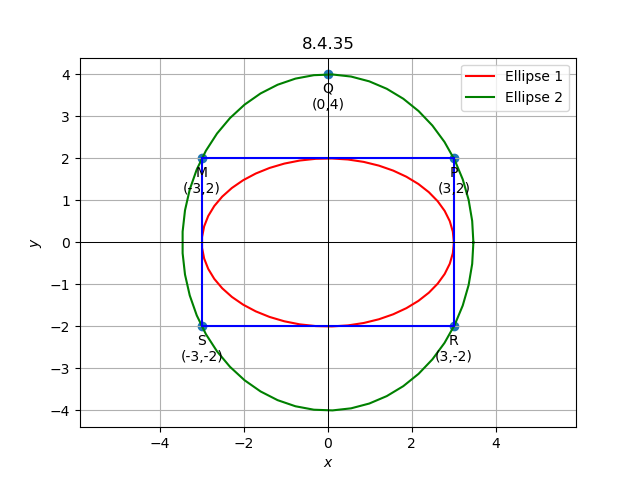
\includegraphics[width=\columnwidth, height=0.8\textheight, keepaspectratio]{../figs/graph2.png}   
\end{frame}


\end{document}
